%\begin{center}
%\huge\bf \underline{ФИЗИКА (Общая физика)}\\[5mm]
%\Large\sl Вячеслав Георгиевич ЕГОРОВ\\
%{\color{blue}(egorov@nusun.jinr.ru)}\\[10mm]
%\sf\LARGE
%2 семестра
%\end{center}

\section{Обзор (план) курса}
%\sf\LARGE
\begin{enumerate}
\item{\underline{\bf Физические основы механики}}

кинематика, динамика, понятие о работе и энергии, законы сохранения, силы тяготения, движение твердого тела и жид\-кости, основные положения СТО
\item{\underline{\bf Молекулярная физика}}

идеальный и реальный газы, распределения Максвелла и Больцмана, основы термодинамики, циклические процес\-сы, явление переноса, молекулярные явления в жидкостях и твердых телах

\item{\underline{\bf Колебания и волны}}

гармонический осциллятор, затухающие и вынужденные ко\-лебания, гармоники, гармонический анализ, волновые явле\-ния, принцип Гюйгенса, интерференция, дифракция, аку\-стические явления, фононы
\item{\underline{\bf	Электричество и магнетизм}}

электростатика, диэлектрики, законы постоянного тока, тер\-моэлектрические явления, ток в электролитах и газах, маг\-нитное поле тока, отклонение заряженных частиц в полях, индукция, электромагнитные колебания и волны

%\newpage
\item{\underline{\bf	Оптика}}

основные свойства света, волновая оптика (поляризация, интерференция и дифракция), прохождение света через ан\-изотропные и движущиеся вещества, голография, термоди\-намика излучения (световой поток, черное тело), лучевая оптика, фотоны

\item{\underline{\bf	Атомная физика}}

строение атомов и молекул, ионизация и диссоциация, боро\-вские орбиты, оптические переходы, правила отбора, спек\-троскопия, лазеры, лазерная спектроскопия, характеристи\-ческое рентгеновское излучение, рентгено-флуоресцентный анализ, масс-спектрометрия

\item{\underline{\bf	Ядерная физика}}

альфа-, бета-, гамма-процессы, ядерные реакции, взаимо\-действие излучений с веществом, детекторы ядерных излу\-чений, ядерные методы исследования материалов ("мече\-ные атомы", нейтроно-акти\-вационный анализ, ядерный ма\-гнитный резонанс)

\end{enumerate}

% \newpage
\section{Ошибки измерений}
 %\centerline{\underline{\huge\bf Ошибки %измерений}}\vspace{5mm}

 Абсолютные ($X =10\pm1$) и относительные ($\Delta X/X=10\%$)\vspace{4mm}

 Симметричные ($X =10\pm1$) и асимметричные ($X=10^{+2}_{-1}$)\vspace{4mm}

 Статистические (уменьшаются с ростом числа измерений) и \vspace{4mm}

 систематические (зависят от метода измерений)\vspace{4mm}

 Написание: 0.01234$\pm$0.00050 или 0.01234(50) или 0.01234$_{\it 50}$\vspace{4mm}

 Меряем 5 раз ширину стола: 1000, 1001, 999, 1000, 1001 мм.\vspace{5mm}

 Среднее значение:
 \begin{displaymath}
\overline{x} = \frac{1000 + 1001 + 999 + 1000 + 1001}{5} = 1000.2
 \end{displaymath}

 Дисперсия (разброс):
 \begin{displaymath}
\sigma \simeq \sqrt{\overline{\left( x_i-\overline{x} \right)^2}}
 \end{displaymath}
 \begin{displaymath}
(-0.2)^2 +(0.8)^2 + (-1.2)^2 + (-0.2)^2 + (0.8)^2 = 2.80
 \end{displaymath}
 \begin{displaymath}
\sigma \simeq \sqrt{(2.80/5)}=\sqrt{0.56} \simeq 0.75
 \end{displaymath}
 \begin{displaymath}
X = 1000.20\pm 0.75 \;\;(67\%CL)
 \end{displaymath}

Смысл дисперсии: с вероятностью 67\% каждое следующее измерение будет попадать в диапазон от 999.45 до 1000.95. Можно показать, что при большой статистике
\begin{displaymath}
X = \overline{x}\pm 2\sigma \;\;(95\%CL)\;\;\;\;\;\;X = \overline{x}\pm 3\sigma \;\;(99.7\%CL)
 \end{displaymath}

Если измерения имеют разную погрешность: 1000$\pm10$, 1001$\pm1$, 999$\pm1$, 1000$\pm1$ и 1001.0$\pm0.1$, то ищем \underline{среднее взвешенное}. \\
Вес i-ой точки: $p_i = \left(\Delta x_i\right)^{-2}$. Чем точнее -- тем больше вес.  Таким образом, веса равны 0.01, 1, 1, 1 и 100.
 \begin{displaymath}
\overline{X}=\frac{\sum_i p_ix_i}{\sum_i p_i}=1000.97;\;\;\;\;\;
\sigma=\sqrt{\frac{\sum_i p_i\left(x_i-\overline{x}\right)^2}{\sum_i p_i}}=0.22
 \end{displaymath}
%\newpage

Измеряем энергию $\gamma$-линии 1460.822(6) кэВ $^{40}$K (Рис.~\ref{fig:k40_spk}) с помощью HPGe детектора и АЦП со шкалой 1 кэВ на канал:

 \begin{figure}[ht]
\centering
 \includegraphics[width=0.95\textwidth]{GP001/GP001F01.eps}
 
% \begin{picture}(165,100)(0,0)
% \put(0, 0){\includegraphics{GP001/GP001F01.eps}}
% \end{picture}
  \caption{Спектр $\gamma$-линии 1460.822(6) кэВ $^{40}$K, измеренной со статистикой 100 (а) и 1M (б) событий.}
   \label{fig:k40_spk} % Метка для ссылки на картинку
\end{figure}

 \begin{displaymath}
 \begin{array}{cclcll}
 a)&\hspace{5mm}&\overline{E} = \frac{1\cdot1453 + 5\cdot1455 +  \ldots
 + 1\cdot1469}{100}           & = 1460.76  &\hspace{5mm}&\sigma = 3.17\\
 b)&            &\overline{E} & = 1460.822 &            &\sigma = 3.066
 \end{array}
  \end{displaymath}

  Ошибка среднего значения:

 \begin{displaymath}
    \Delta(\overline{X}) = \overline{(\overline{X}-X_0)}\;\;\simeq\;\; \frac{\sigma}{\sqrt{N}}
 \end{displaymath}
 \begin{displaymath}
  \begin{array}{lclcl}
   \overline{E}_{(N=100)}     &=& 1460.76  & \pm & 0.32\\
   \overline{E}_{(N=1000000)} &=& 1460.822 & \pm & 0.003
  \end{array}
 \end{displaymath}
 
С увеличением статистики дисперсия не изменилась, но ошибка уменьшилась!
 \\[3mm]

\underline{Если измерение величины $\phi$ не прямое:} $\;\;\;\phi = f(x\pm\Delta x,y\pm \Delta y)$
 \begin{displaymath}
(\Delta\phi)^2 = \left(\frac{\partial f}{\partial x}\cdot\Delta x\right)^2 +
                 \left(\frac{\partial f}{\partial y}\cdot\Delta y\right)^2
 \end{displaymath}
(ошибка результата $\Delta\phi$)$^2$ = (ошибка из-за $\Delta x$)$^2$ + (ошибка из-за $\Delta y$)$^2$.\\ Производная $\frac{\partial f}{\partial x}$ -- это  {\em коэффициент влияния} параметра $x$ на функцию $f$.
%\newpage

\section{Метод Наименьших Кавдратов (Least Squares)}
%{\Huge Метод Наименьших Кавдратов (Least Squares)}\\[3mm]

Задача: фитировать набор N экспериментальных точек ($x_i,y_i$) какой-то
функцией $Y=f(X)$. LS-критерий -- малость остаточной суммы $\chi^2$.

 \begin{displaymath}
\chi^2 = \sum_{i=1}^N p_i\left[y_i - f(x_i)\right]^2;\;\;\;\;\;\;\;\;\;\;
p_i = \frac{1}{\left(\Delta y_i\right)^2}\;\;.
 \end{displaymath}
 
Примеры фитирующих функций с 1 или 2 параметрами показаны на Рис.~\ref{fig:fit_fun}.

 \begin{figure}[htp] 
 \setlength{\unitlength}{1mm}
 \begin{picture}(165,180)(0,0)
 \put(10, 0){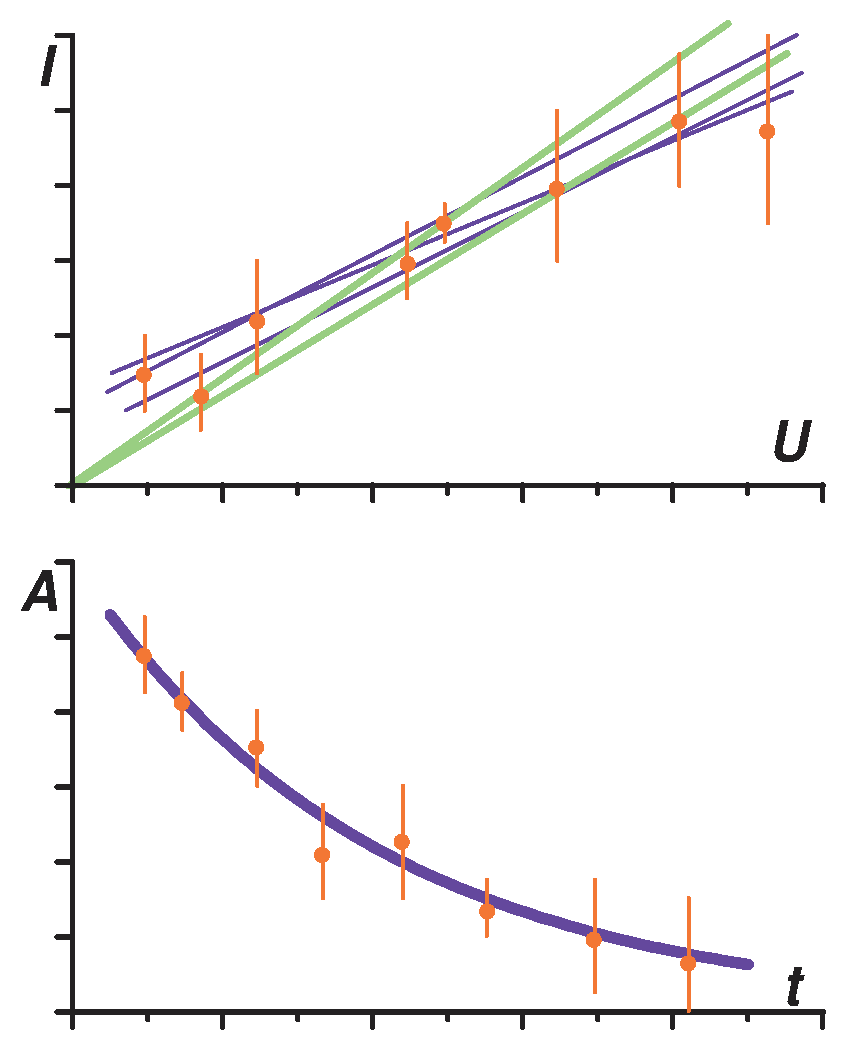
\includegraphics{GP001/GP001F02.eps}}
 \put(25, 165){\makebox(0,0)[l]{\Large\sf Вольт-амперная характеристика}}
 \put(48, 155){\makebox(0,0)[c]{\color{blue}\Huge\bf $I=aU+b$}}
 \put(22, 146){\makebox(0,0)[l]{\color{blue}\Large\bf (какая-то прямая,}}
 \put(22, 141){\makebox(0,0)[l]{\color{blue}\Large\bf надо найти $a$ и $b$)}}
 \put(120, 125){\makebox(0,0)[c]{\color{green}\Huge\bf $I=U/R=k\cdot U$}}
 \put(110, 115){\makebox(0,0)[c]{\color{green}\Large\bf (прямая проходит через О, }}
 \put(110, 109){\makebox(0,0)[c]{\color{green}\Large\bf надо найти наклон $k=1/R$)}}
 \put( 40,  70){\makebox(0,0)[l]{\Large\sf Закон радиоактивного распада}}
 \put(110,  57){\makebox(0,0)[c]{\color{blue}\Huge\bf $A=A_0\cdot e^{-t/\tau}$}}
 \put(105,  47){\makebox(0,0)[c]{\color{blue}\Large\bf (экспонента; надо найти $A_0$ и $\tau$)}}
 \end{picture}
\caption{Примеры фитирования вольт-амперной характеристики (вверху) и данных радиоактивного распада (внизу).}
   \label{fig:fit_fun} % Метка для ссылки на картинку
\end{figure}
 
%\newpage

Итак, надо найти такие значения двух параметров ($A_0$ и $\tau$), чтобы остаточная сумма $\chi^2$ была ми\-ни\-мальной. Условие минимума:

 \begin{displaymath}
\frac{\partial(\chi^2)}{\partial A_0}=0\;\;\;;\;\;\;\;\;\;
\frac{\partial(\chi^2)}{\partial \tau}=0\;\;.
 \end{displaymath}
 \begin{displaymath}
 \left\{
 \begin{array}{cc}
 \sum_i p_i \left[y_i-f(t_i)\right]\frac{\partial f(t_i)}{\partial A_0} &= 0\\[2mm]
 \sum_i p_i \left[y_i-f(t_i)\right]\frac{\partial f(t_i)}{\partial \tau} &= 0
 \end{array}
 \right|\;\;\;\;\;\;\Rightarrow\;\;\;A_0,\;\;\tau
 \end{displaymath}

Если сложный вид $f(x)$ и число параметров $K\gg 1$, то система не решается. Тогда используем \underline{топографический метод}: составляем как бы {\sl карту высот} $\chi^2$ на k-мерной плоскости и ищем на ней низину (Рис.~\ref{fig:2d_fit_surf}).

\begin{figure}[htp] 
 \setlength{\unitlength}{1mm}
 \begin{picture}(165,80)(0,0)
 \put(0, 0){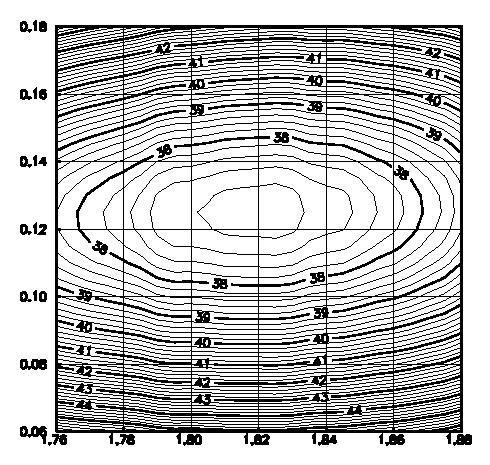
\includegraphics{GP001/GP001F03.eps}}
 \put(85, 0){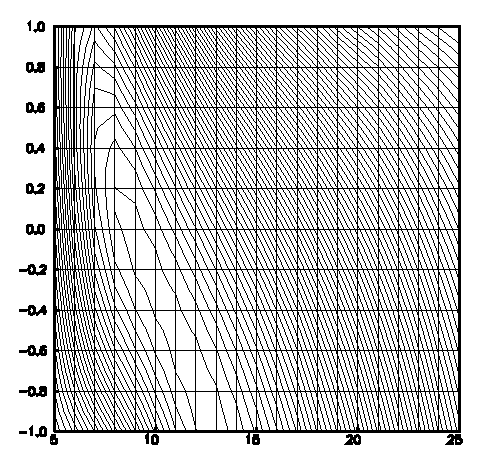
\includegraphics{GP001/GP001F04.eps}}
 {\color{red}
 \put(20,15){\vector(1,4){4}}
 \put(24,31){\vector(1,1){10}}
 \put(34,41){\vector(1,0){6}}
 \color{black}}
 \end{picture}
  \caption{2D-поверхности в фазовом пространстве фитируемых параметров.}
   \label{fig:2d_fit_surf} % Метка для ссылки на картинку
\end{figure}

\underline{Градиентный метод} (то же самое, но низина ищется автоматически). Суть: искомые параметры выбираются наугад (на k-мерной плоскости ставится точка), а затем для этой точки  ищется градиент, то есть, {\color{red}вектор}, показывающий на\-правление максимального изменения $\chi^2$. Находится новая точка, и т. д.  Стандартный программный пакет MINUIT.\\

Свойства  $\chi^2$
\begin{itemize}
\item если "покачать" параметр A на $\pm\Delta A$, то $\chi^2$ увеличится на +1.0
\item нормированное $\chi^2_{\rm norm}=\chi^2/(N-K)$ должно быть $\simeq1$.

Если $\chi^2_{\rm norm}>1$, то неверный вид функции или $\exists$ систематика.

Если $\chi^2_{\rm norm}<1$, то погрешность каждой точки слишком велика.
\end{itemize}
%\newpage

\section{Максимальное Правдоподобие (Maximal Likelyhood)}
%{\color{green}
%{\Huge Максимальное Правдоподобие (Maximal Likelyhood)}\\
%\underline{(Это -- пока вне программы; просто знайте, что %существует и такой метод)}
%}

Если в качестве фитируемых точек используется не измеренная каким-то прибором аналоговая величина $Y_i\pm\Delta Y_i$, а число событий $N_i(X)$ (например, число $\gamma$-квантов, зарегистрированных детектором), то как быть с погрешностью $\Delta N_i$ и весом точек? При больших $N$ погрешность
$\Delta N\simeq\sqrt{N}$, а при малых -- ?...

ML-критерий: надо так подобрать параметры фитирующей функции $f(x)$, чтобы была максимальной вероятность получить в эксперименте именно те точки, которые в нем и получились.

\begin{figure}[ht]
 \setlength{\unitlength}{1mm}
 \begin{picture}(165,90)(0,0)
 \put(0,5){\includegraphics{GP001/GP001F05.eps}}
 \end{picture}
\caption{Распределение пуассона с параметрами задачи в тексте.}
   \label{fig:poisson} % Метка для ссылки на картинку
\end{figure}

\underline{Распределение Пуассона}

Например, мы знаем, что через 1 дм$^2$ пролетает в среднем $\lambda=1.5$ мюона в секунду. Какова вероятность того, что за данную конкретную секунду мы увидим N=1 мюон? N=2 мюона? N=0 мюонов (Рис.~\ref{fig:poisson})? 
\begin{displaymath}
p(N)=\frac{\lambda^N}{N!}e^{-\lambda}
\end{displaymath}


ML-критерий:

\begin{displaymath}
\Phi =\left.\prod_i\frac{\left[f(\overrightarrow{R},x_i)\right]^{N_i}}{N_i!}\cdot e^{-f(\overrightarrow{R},x_i)}\;\right\}\;\;\;\rightarrow\;\max
\end{displaymath}

\section{Литература}
%\newpage
\sf\Large
\renewcommand{\bibname}{}
\phantomsection
\begin{thebibliography}{99}
\bibitem{Фриш}
С.Э.Фриш и А.В.Тиморева, {\bf Курс общей физики}, 3 тома. {\sl\large (ГУ)}\\
{\large
I том: Физические основы механики. Молекулярная физика. Колебания и волны.\\
II том: Электрические и электромагнитные явления.\\
III том: Оптика. Атомная физика.
}
\bibitem{Иродов}
И.Е.Иродов, {\bf Общая физика}. 5 томов {\sl\large (без нумерации. МИФИ.)}\\
{\large
{\sl Механика. Основные законы}.\\
{\sl Физика макросистем. Основные законы}.\\
{\sl Волновые процессы. Основные законы}.\\
{\sl Электромагнетизм. Основные законы}.\\
{\sl Квантовая физика. Основные законы}.
}
\bibitem{Савельев}
И.В.Савельев, {\bf Курс физики}. {\sl\large (3 тома. МИФИ.)}\\
{\large
I том: Механика. Молекулярная физика. \\
II том: Электричество. Колебания и волны. Волновая оптика.\\
III том: Квантовая оптика. Атомная физика. Физика твердого тела. Ядро и частицы.
}
\bibitem{Сивухин}
Д.В.Сивухин, {\bf Курс общей физики}.  {\sl\large (5 томов. МФТИ, Физфак СПбГУ.)}\\
{\large
I том: Механика.\\
II том: Термодинамика и молекулярная физика. \\
III том: Электричество. \\
IV том: Оптика.\\
V том: Атомная и ядерная физика.
}
\bibitem{Калашников}
С.Г.Калашников, {\bf Электричество}.
\bibitem{Тамм}
И.Е.Тамм, {\bf Основы теории электричества}.
\bibitem{Калитеевский}
Н.И.Калитеевский, {\bf Волновая оптика}.
\bibitem{Шпольский}
Э.В.Шпольский, {\bf Атомная физика}.
\bibitem{Борн}
М.Борн, {\bf Атомная физика}.
\bibitem{Мухин}
К.Н.Мухин,  {\bf Экспериментальная ядерная физика}. {\sl\large (2 тома).}
\end{thebibliography}


